\section{Вивчаємо фізику за допомогою Scratch}

\Authors{Мізюк Олександр Миколайович}
\aff{Механіка. Вільне падіння і криволінійний рух під дією незмінної сили тяжіння}
\AbsKeywords{У цьому розділі представлений зразок розв'язування задачі на рух тіла кинутого під кутом до горизонту. Для моделювання процесу руху використовуйте застосунок, створений у середовищі програмування \href{https://scratch.mit.edu/projects/editor/?tutorial=getStarted}{Scratch}.
}{Ключові слова}{механіка, криволінійний рух, Scratch, \LaTeX}

\subsection{Рух тіла, кинутого під кутом до горизонту}

Прочитавши про рекорди швидкості польоту спортивних снарядів, учениця Оленка вирішила з’ясувати, якої швидкості вона надає футбольному м’ячу. Для цього дівчинка вдарила по м’ячу, спрямувавши його під кутом \textbf{$45^{\circ}$} до горизонту (див. мал. \ref{fig:hit1}).

\begin{figure}[h]
	\centering
	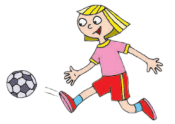
\includegraphics[width=0.3\linewidth]{./images-miziuk/hit1.png}
	\caption{
		\centering
		За напрямком і дальністю польоту м’яча ви можете визначити, якої швидкості ви надали м’ячу під час удару або кидка.}
	\label{fig:hit1}
\end{figure}

М’яч упав на землю на відстані \textbf{40 м} від учениці. Виконавши розрахунки, дівчинка вирішила, що вона надала м’ячу швидкості \textbf{20 м/с}, а м’яч піднявся на висоту \textbf{8 м}. Чи не помилилася учениця?

\subsection{Розв'язуємо задачу\protect\footnote{Ознайомтеся з розв’язанням задачі. Скориставшись отриманими формулами, оцініть розрахунки дівчинки, а після уроків проведіть подібний експеримент та оцініть швидкість, якої ви надаєте м’ячу.}}

Футболістка вдарила по м’ячу, надавши йому швидкості $v_0$, напрямленої під кутом $\alpha$ до горизонту. Визначте дальність польоту та найбільшу висоту підйому м’яча.

\begin{center}
	\begin{tabular}{|l|l|} 
		\hline
		Дано & \textit{Розв'язання} \\
		\hline
		$v_0$ & \\
		$\alpha$ & \\
		$g$ & \\	
		\hline
		$L - ?$ & \\
		$h_{max} - ?$	& \\
		\hline
	\end{tabular}
\end{center}

Виконаємо пояснювальний рисунок (див. мал. \ref{fig:hit2}): початок координат пов’яжемо з точкою на поверхні Землі, де м’яч відірвався від бутси футболістки; вісь \textbf{OY} спрямуємо вертикально вгору; вісь \textbf{ОХ} — горизонтально.

\begin{figure}[h]
	\centering
	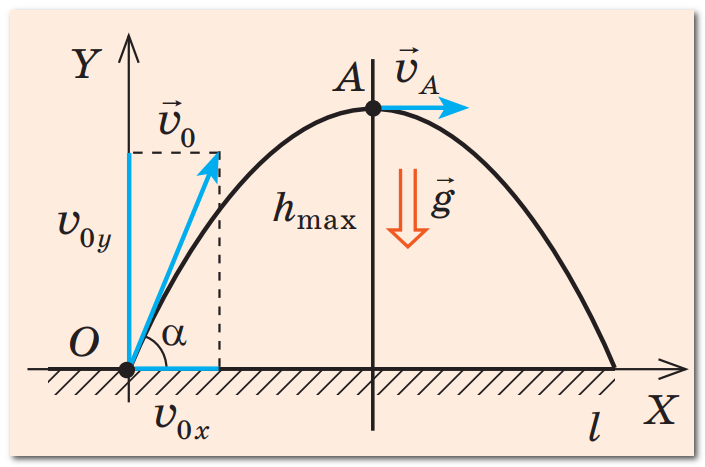
\includegraphics[width=0.6\linewidth]{./images-miziuk/hit2.png}
	\caption{
		\centering
		Пояснювальний рисунок.}
	\label{fig:hit2}
\end{figure}

В обраній системі відліку:

рух уздовж осі \textbf{ОХ} — рівномірний:

\begin{equation}\label{eq:hinteq1}
	v_x = v_{0x}, x = x_0 + v_{0x}t,
\end{equation}

де 

$$
	x_0 = 0, v_{0x} = v_0cos\alpha 
$$

рух уздовж осі \textbf{ОY} — рівноприскорений:

\begin{equation}\label{eq:hinteq2}
	v_y = v_{0y} + g_yt, y = y_0 + v_{0y}t + \dfrac{g_yt^2}{2},
\end{equation}

де 

$$
	y_0 = 0, v_{0y} = v_0sin\alpha, g_y = -g,
$$

тому рівняння \eqref{eq:hinteq1} і \eqref{eq:hinteq2} набувають вигляду:

\begin{equation}\label{eq:hinteq3}
	v_x = v_0cos\alpha, x = v_0cos\alpha\cdot t
\end{equation}

і

\begin{equation}\label{eq:hinteq4}
	v_y = v_0sin\alpha - gt, y = v_0sin\alpha\cdot t - \dfrac{gt^2}{2}
\end{equation}

відповідно. Час \textbf{t1} руху м’яча до верхньої точки траєкторії (точки \textbf{А}) знайдемо з умови: $v_y(t_1) = 0$:

\begin{equation}\label{eq:hinteq5}
	v_0sin\alpha - gt_1 = 0 \Rightarrow t_1 = \dfrac{v_0sin\alpha}{g}.
\end{equation}

Координата y м’яча в точці \textbf{А} — це максимальна висота підйому м’яча:

\begin{equation}\label{eq:hinteq6}
	h_{max} = y_A = v_0sin\alpha\cdot t_1 - \dfrac{gt_1^2}{2}.
\end{equation}

Після підстановки \textbf{t1} отримуємо формули для визначення максимальної висоти підйому та загального часу руху м’яча:

\begin{equation}\label{eq:hinteq7}
	h_{max} = \dfrac{v_0^2sin\alpha^2}{2g};
\end{equation}

\begin{equation}\label{eq:hinteq8}
	t = 2t_1 = \dfrac{2v_0sin\alpha}{g}.
\end{equation}

Дальність \textbf{L} польоту дорівнює координаті \textbf{х} тіла наприкінці руху (\textbf{x = L}):

\begin{equation}\label{eq:hinteq9}
	x = v_0cos\alpha\cdot t = v_0cos\alpha\cdot \dfrac{2v_0sin\alpha}{g}. 
\end{equation}

Отже, дальність польоту:

\begin{equation}\label{eq:hinteq10}
	2cos\alpha\cdot sin\alpha \Rightarrow L = \dfrac{v_0^2sin2\alpha}{g}. 
\end{equation}

\begin{figure}[h]
	\centering
	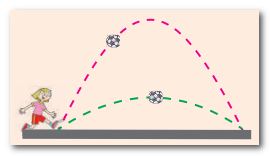
\includegraphics[width=0.6\linewidth]{./images-miziuk/hit3.png}
	\caption{
		\centering
		Однакова дальність польоту при різних траєкторіях.}
	\label{fig:hit3}
\end{figure}

\textbf{Зверніть увагу!} З останньої формули випливає:

\begin{itemize}
	\item якщо кинути тіло під кутом $\alpha$, а потім під кутом $90^{\circ} - \alpha$, то дальність польоту не зміниться, тобто тіло потрапить у ту саму точку, рухаючись різними траєкторіями (див. мал. \ref{fig:hit3})
	\item максимальної дальності польоту тіло сягає, якщо $\alpha = 45^{\circ}$ ($sin2\alpha = 1$).
\end{itemize}

\subsection{Моделювання руху у Scratch}

\begin{figure}[h]
	\centering
	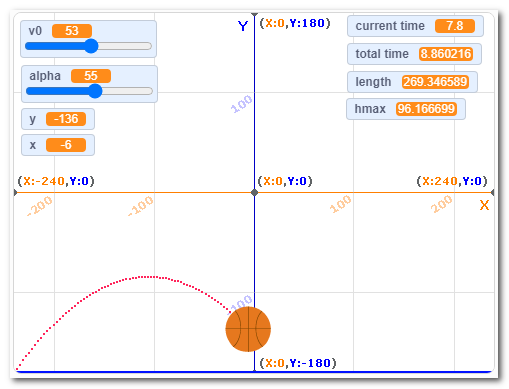
\includegraphics[width=1\linewidth]{./images-miziuk/hit4.png}
	\caption{
		\centering
		Знімок вікна проєкту.}
	\label{fig:hit4}
\end{figure}

Щоб розглянути код проєкту, \href{https://scratch.mit.edu/projects/681697866}{перейдіть за покликанням}. 

\subsection{Підбиваємо підсумки}

Траєкторія руху тіла, кинутого під кутом до горизонту, - параболічна. Такі рухи розглядають як результат додавання двох простих рухів: горизонтального - рівномірного уздовж осі \textbf{OX} і вертикального - рівноприскореного (з прискоренням \textbf{g}) уздовж осі \textbf{OY}. 

Рівняння залежностей проекції швидкості та координати від часу у цьому разі мають вигляд:

$$
	v_x = v_{0x}, 
$$

$$
	x = x_0 + v_{0x}t,
$$

$$
	v_y = v_{0y} + g_yt, 
$$

$$
	y = y_0 + v_{0y}t + \dfrac{g_yt^2}{2}.
$$

\subsection{Контрольні запитання}

\begin{itemize}
	\item Який вигляд має рівняння руху, якщо тіло кинуто під кутом до горизонту?
	\item Якою є траєкторія руху тіла, кинутого під кутом до горизонту? Наведіть приклади.
	\item Як визначити модуль і напрямок швидкості руху тіла в будь-якій точці траєкторії?
\end{itemize}

\subsection{Вправа для самостійного розв'язування}

Опором повітря нехтуйте. Вважайте, що $g = 10 {}^2$ % 
{м/с}.\\

Струмінь води, напрямлений під кутом \textbf{$60^{\circ}$} до горизонту, сягнув висоти \textbf{15 м}.

\begin{enumerate}
	\item Використайте розроблений Scratch-проєкт для дослідження руху струменя води.
	\item Знайдіть: 
	\begin{enumerate}
		\item швидкість витікання води; 
		\item час польоту частинок струменя; 
		\item дальність польоту частинок струменя.
	\end{enumerate}
	\item Якою буде дальність струменя, якщо спрямувати його під кутом \textbf{$30^{\circ}$} до горизонту?
	\item Чому струмінь води розширюється?	
\end{enumerate}